
\chapter{Image file formats and steganography techniques}

\section{Introduction}

\setlength\columnsep{20pt}
\begin{multicols}{2}
An image is a two-dimensional representation depicting any possible subject conceivable by human imagination, captured using an optical device (such as a camera or a telescope) or a natural object (human eyes). The image can then be rendered and displayed for other people to see either manually (by painting, carving etc.) or automatically (by using a computer). In this chapter we will focus on images captured using digital optical devices that are rendered automatically. The correct term for them is digital images, but throughout the rest of the paper they will be reffered to as images for convenience.

\begin{figure}[H]
    \centering
    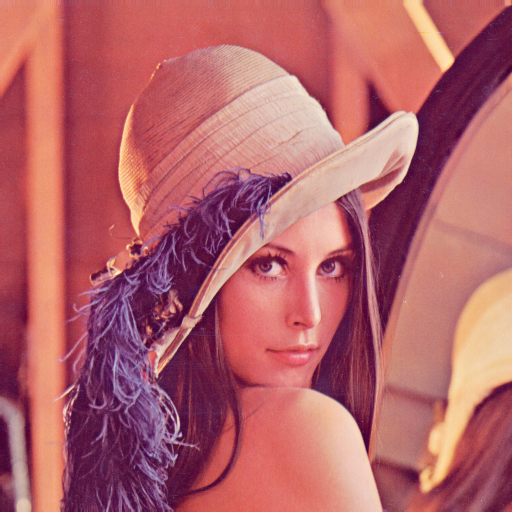
\includegraphics[width=5cm,height=5cm,keepaspectratio]{pics/lenna}
    \caption{Lenna - Classic example of a digital image}
    \label{Lenna}
\end{figure}

Computers are programmed to do operations in a clear sequential way and this rule doesn't change when working with pictures. In order for a computer to be able to render an image, it needs to know some general metadata information about the photo, such as the width and height, as well as the data bytes of the image. These bytes are the actual representation of the picture which compose the two-dimensional pixel map\footnote{This is true for a lossless format, where each pixel is stored in memory. It is not exactly the case for lossy formats such as JPEG where the image goes through processing before being rendered. More information later in the chapter.}. A pixel is the smallest unit that a computer monitor can read and display. The pixel color is the result of merging the different color channels which compose the picture (such as RGB, YUV, YCbCr etc.). Here is an example of the entire process - let's assume that from the image data bytes the first 3 bytes have the decimal values 20, 127, 250 and that it uses the RGB color model. This means that when the computer will have to render the image, the first pixel will have the red component equal to 20 (0x14), the green equal to 127 (0x7F), and the blue equal to 250 (0xFA), in what will finally be interpreted as \#147FFA by the monitor (variation of light blue). 

\begin{figure}[H]
    \centering
    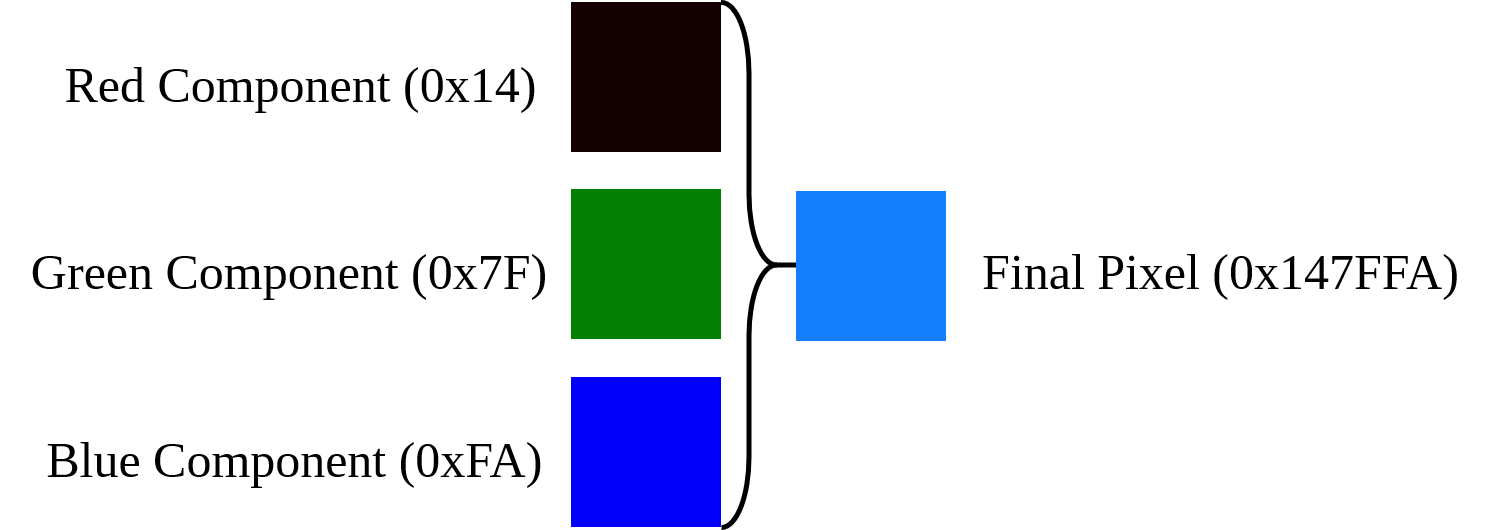
\includegraphics[width=8cm,height=2.15cm,keepaspectratio]{pics/how_a_pixel_works}
    \caption{How 3 colors channels build the pixel}
    \label{Pixel Creation}
\end{figure}

By merging multiple pixels over a two-dimensional space, they will eventually start to resemble an image that can be stored on a disk as a byte stream and can be rendered anytime by parsing the aforementioned stream. Each pixel can be represented as a point in that space with coordinates that are part of the unsigned integer domain. An entire row of pixels, i.e. pixels that have the same ordinate value, is sometimes also referred to as a scanline because in the earlier days of modern computing, computers would be given the width of the image and based on that value they would read a precise amount of bytes and render it on the screen before moving on to the next scanline, repeating this process until there would be no more information.

It is important to note that most of these developments have been done in a time where the maximum storage was extremely limited and not very fast, very different from what it is today. In order to save some space they looked into different compression algorithms to apply to the byte streams and today they fall into two distinict categories: the lossless algorithms are the ones that compress all the original information without destroying any of it, while on the other hand there are the lossy algorithms which are able to identify which information is useless and delete it accordingly. This concept also applies to file formats and we will see in later chapters more concrete examples. 

With all of this information in mind, we can now procede to discussing the most commonly formats commonly used in today's.

\section{BitMap Picture (BMP)} \label{BMP_Explained_Chapter}

The BMP file format, also known as the device independent bitmap file format(DIB), bitmap image file or just bitmap, is a lossless\footnote{It is true that the format specification standards supports compression but further research reveals that currently it only supports lossless types of compression, such as the Huffman or Run Length Encoding algorithms.} image file format originally designed by Microsoft back in 1986 in order to store two-dimensional digital images on their Windows operating system. Over the years it has developed plenty of variations and extensions that were based on the original specification but this paper will focus only on the most common available ones, no extended versions that are looking to improve the format since they do not add anything interesting or new to the way the format stores the data thus affecting the steganography algorithms.

As with almost every file format, the final BMP byte stream can be seen as a result of the merge between the BMP header which contains metadata about the file and the BMP data which is the actual pixel information. As we can see from table \ref{BMP_Header_Table}, the BMP header stores a lot of important information about the image that is useful for any rendering software while making sure to allocate enough memory to be able to display the picture on the screen and other essential steps. It is also important to note that all the structures seen in the BMP header use the little-endian format for representation and are usually more troublesome on the systems that have the default set as big-endian.
\end{multicols}

 \begin{center}
	\begin{tabular}{|l|l|l|l|}
		\hline
		\textbf{Information} & \textbf{Size} & \textbf{Offset} & \textbf{Description} \\ \hline
		Signature & 2 bytes & 0x00 & Two chars, 'B' and 'M' \\ \hline
		File size & 4 bytes & 0x02 & Total file size in bytes \\ \hline
		Reserved & 4 bytes & 0x06 & Unused space \\ \hline
		Data offset & 4 bytes & 0x0A & Offset to get to the actual BMP data \\ \hline
		Size & 4 bytes & 0x0E & Size of the left header information \\ \hline
		Width & 4 bytes & 0x12 & Horizontal size of the image \\ \hline
		Height & 4 bytes & 0x16 & Vertical size of the image \\ \hline
		Planes & 2 bytes & 0x1A & Amount of image planes \\ \hline
		Bits Per Pixel & 2 bytes & 0x1C & How many bits are used to represent each pixel \\ \hline
		Compression & 4 bytes & 0x1E & Indicates the type of compression used \\ \hline
		Image size & 4 bytes & 0x22 & The size of the compressed image, can be 0 \\ \hline
		X pixels per Meter & 4 bytes & 0x26 & Horizontal resolution in pixels/meter \\ \hline
		Y pixels Per Meter & 4 bytes & 0x2A & Vertical resolution in pixels/meter \\ \hline
		Colors Used & 4 bytes & 0x2E & \begin{tabular}[c]{@{}l@{}}Number of actually used colors\\ (based on Bits Per Pixel)\end{tabular} \\ \hline
		Important Colors & 4 bytes & 0x32 & Number of important colors (usually all) \\ \hline
	\end{tabular}
	\label{BMP_Header_Table}
 \end{center}

\begin{multicols}{2}
Analyzing the obligatory BMP header fields we realise that most of them are useless for any steganographic purposes mainly because they can't be altered without having major consequences on the renderer software but there are still a few interesting ones left:
\begin{itemize}
  \item The 4 bytes that are reserved and unused could be very well put to use by using the methods presented in chapter \ref{Unused_Space_Chapter}, so we can use either this space to send parts of a message over multiple BMP files, or we can store the secret message size in these 4 bytes and write the secret after the actual image data has ended.
  \item Data offset could be useful because some renderers use this field to indicate the offset of the actual image data and just skip any other irelevant metadata information, allowing us to hide information in those fields.
  \item The width and the height of the image usually are altered to hide bottom parts of the image that may contain hidden information or by masking the result of the merge of two images and just showing the top one. Let's take for example this image of the sun that is obviously missing a part for demonstration purposes.

\begin{figure}[H]
    \centering
    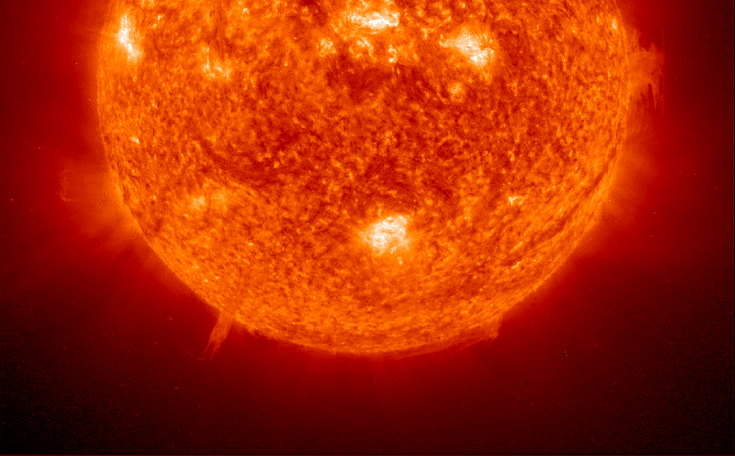
\includegraphics[width=4cm,keepaspectratio]{pics/height_modification_steganography_cut}
    \caption{Incomplete sun image}
    \label{Sun_Missing_Part}
\end{figure}

However if we adjust by trial and error the height of the image to see if there is any more bytes to render, we would notice that there really is a message hidden with those bytes that some steganalysis softwares would detect but any renderer software such as the Windows Media Viewer would always miss. In other words, we have tricked the software to not display more scanlines than we wanted it to display, even though the information is there, not corrupted in any way.

\begin{figure}[H]
    \centering
    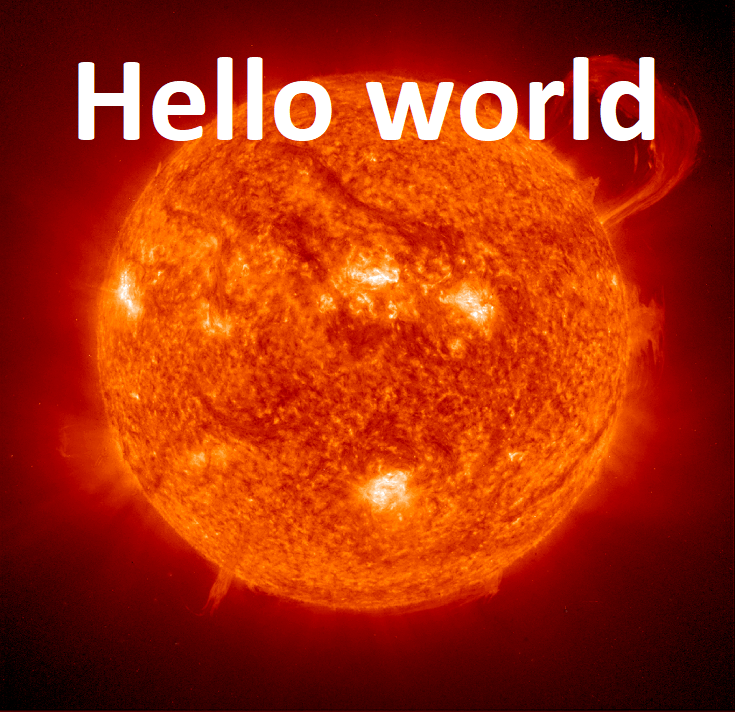
\includegraphics[width=4cm,keepaspectratio]{pics/height_modification_steganography_original}
    \caption{Complete sun including the hidden message}
    \label{Sun_Original}
\end{figure}
\end{itemize}

Moving on from the metadata block of the BMP format to the actual data byte stream, we find additional interesting information about how the pixel data is actually stored. Most images use the Red, Green and Blue also known as RGB values to compose the final pixel color, but for an unknown reason the creators of the bitmap format decided to store the information in the reverse order in the data stream as Blue, Green, Red or BGR. However this is not the only change they made from the other common image formats available at the time: rather than storing the scanlines from a top to down order, BMP decided to store them bottom-up.

\begin{figure}[H]
    \centering
    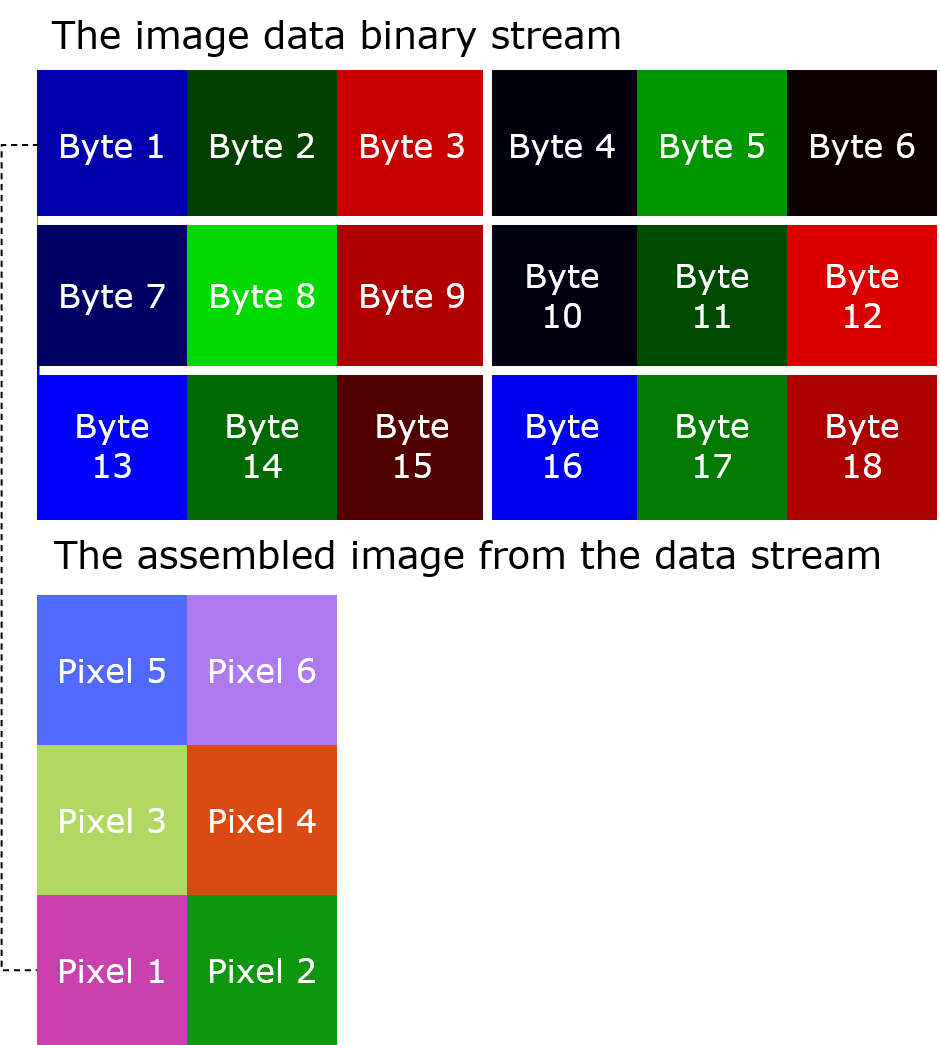
\includegraphics[width=7cm,keepaspectratio]{pics/assembling_bmp_image}
    \caption{How the BMP image is rendered}
    \label{bmp_how_to_render}
\end{figure}

This behaviour can be noticed in figures \ref{Sun_Missing_Part} and \ref{Sun_Original} where the top part is cropped in order to hide a message and we can now understand why it is only that part that can be made redundant in the steganography process: because the last bytes of the image data binary stream are actually responsible for the rendering of the top section of the picture. Seeing and understanding how the carrier format works is the first and most important step in embedding messages in a covert way.

\subsection{Image sub-block scrambling using the BMP format}
Sub-block scrambling is a type of scrambling algorithm, like those introduced in chapter \ref{scrambling_chapter}, that can be applied to images stored in the BMP format. It was created by the author of this thesis based on the idea of the JPEG format and the algorithm it uses during compression that is applied only on sub-blocks of 8x8 size. We mentioned in chapter \ref{scrambling_chapter} that most scrambling algorithms have \[ MMS \leq [CDS \ / \ 8] \ bytes \] but the target was to design and implement an algorithm which can make use of all the bytes available in the cover, and we ended up with this method which has 
\begin{equation} \label{eq:1}
MMS = [CDS \ / \ 8] \ bytes
\end{equation}
 making it similar in storage capacity to a sequential algorithm. That performance was achieved following a simple procedure:
\begin{itemize}
  \item Separate the image into multiple blocks of BLOCK\_SIZE (this is a global constant value which is usually equal to 8 but can be higher or lower). It doesn't matter if the width or height of the image are not a multiple of BLOCK\_SIZE, the algorithm also works with non-square blocks.
  \item The algorithm needs a password to work with in order to use it as a seed when generating a permutation. Each block calls a helper method to obtain the given permutation for itself based on its own width and height. That permutation is the order in which the data will be written.
  \item The first block is reserved for writing the metadata about the message(such as the length of the secret) and the other blocks are for writing the actual contents of the message.
\end{itemize}

\end{multicols}

\definecolor{lightergray}{rgb}{0.92,0.92,0.92}
\lstset{escapeinside={<@}{@>},
		frame=single,
		xleftmargin=-25.4pt,
	      xrightmargin=-25.4pt
}

\begin{lstlisting}[backgroundcolor = \color{lightergray},language=Python,caption={Pseudocode of the scramble algorithm},captionpos=b]
 global constant BLOCK_SIZE;

 procedure embed_subblock(secret, subblock, random_engine)
   #Generate a permutation from 0 to subblock.width * subblock.height
   #using the random_engine given. That permutation will be the order
   #used when writing the secret data into the subblock data.
   writing_order<@$\gets$@>random_permutation(0,subblock.width*subblock.height,random_engine); 

   for each byte_index in writing_order do
     #Getting the absolute index of the subblock rows and 
     #columns where we need to write the secret information.
     subblock_row<@$\gets$@>subblock.starting_line_index+byte_index/subblock.width;
     subblock_column<@$\gets$@>subblock.starting_column_index+byte_index%subblock.width;
     set_least_significant_bit(subblock.data[subblock_row][subblock_column],secret);

     #We move to the next bit of the secret information
     advance_to_next_secret_bit(secret);
		
 procedure pseudo_scramble(cover, secret, password)
   #Creating a new pseudo-random engine with a given seed.
   random_engine<@$\gets$@>new pseudo_random_engine(password);

   for each subblock of cover with subblock.size<@$\leq$@>BLOCK_SIZE
     if subblock = cover.first_subblock
       #Used for hiding the size of the secret into 
       #the first subblock of the cover in an order
       #given by the pseudo-random engine random_engine.
       embed_subblock(secret.size,subblock,random_engine);
     else
       #If it's not the first subblock of the cover, 
       #write the actual secret into the subblock.
       embed_subblock(secret.iterator,subblock,random_engine);

\end{lstlisting}

\begin{multicols*}{2}
It is much easier to explain the algorithm using a simple example, so let's begin with the image represented in figure \ref{scramble_example_original_image}. It is BMP image with a resolution of 10x6 pixels (10 pixels wide, 6 pixels tall). Furthermore, let's also create the parameters needed by the algorithm in order to embed a message:
\begin{itemize}
  \item The secret message we want to hide in the cover file is "Hello World", no quotes.
  \item Given the aforementioned message, we can calculate its size: 5 characters for the word "Hello", 5 characters for "world" and 1 character for the space inbetween. Total message length is 11 characters or 11 bytes using the ASCII standard. 
  \item The password used for generating the seed is "super\_secret\_key", no quotes.
  \item The BLOCK\_SIZE used in splitting the original image is equal to 4.
\end{itemize}

\begin{figure}[H]
    \centering
    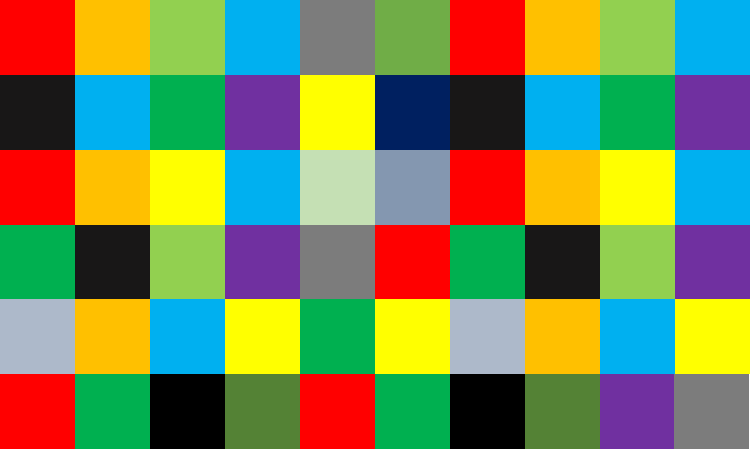
\includegraphics[width=7cm,keepaspectratio]{pics/bmp_scrambling/original_image}
    \caption{Original BMP cover image}
    \label{scramble_example_original_image}
\end{figure}

Knowing all of this information we can already know if the cover file is going to be able to hold the secret message based on the formula \ref{eq:1}. We know that the BMP format uses 3 bytes for storing each pixel and that our image is 10 pixels wide and 6 pixels tall, so we have that 
\\$CDS=3*10*6=180\ bytes \overset{(\ref{eq:1})}{ \implies }\\ \overset{(\ref{eq:1})}{ \implies } MMS=[180/8]=22\ bytes$

Since our total message length is smaller than $MMS$, we know that we will not be running out of cover space during the embedding process. After making these verifications, we can begin by initializing our pseudo-random engine based on the given password meant to be used as a seed and we can also start splitting the original image into sub-blocks, ending up with a result similar to figure \ref{scramble_example_subblocks}. Since neither the width or height of the image are multiples of the BLOCK\_SIZE constant, we have several smaller blocks (to be more precise, blocks 3, 4, 5 and 6) that are still going to be used for embedding purposes. 

\begin{figure}[H]
    \centering
    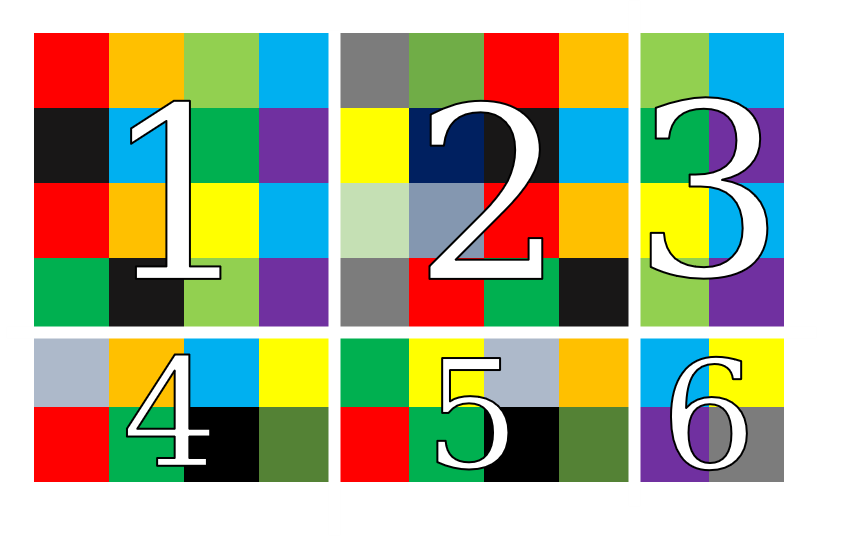
\includegraphics[width=7cm,keepaspectratio]{pics/bmp_scrambling/image_broken_subblocks}
    \caption{Sub-blocks of the original image}
    \label{scramble_example_subblocks}
\end{figure}

\section{Portable Network Graphics (PNG)} \label{PNG_Explained_Chapter}

\section{Joint Photographic Experts Group (JPEG)} \label{JPEG_Explained_Chapter}
\end{multicols*}
